\documentclass[12pt, a4paper, oneside]{ctexart}
\usepackage{amsmath, amsthm, amssymb, bm, color, framed, graphicx, hyperref, mathrsfs, float, caption,subfigure}
\usepackage[justification=centering]{caption}

% multi-column
\usepackage{tasks}
% itemize
\NewTasksEnvironment[label=(\arabic*), label-width=3ex]{exercise}
%\settasks{
% label = \theexercise.\arabic* ,
% item-indent = 2em ,
% label-width = 2em ,
% label-offset = 0pt
%}

\everymath{\displaystyle}

\title{\textbf{第五次作业}}
\author{U08M11002 Fall 2023}
\linespread{1}
\definecolor{shadecolor}{RGB}{241, 241, 255}

\newcounter{problemname}
\newenvironment{problem}{\stepcounter{problemname}\par\noindent\textbf{题目\arabic{problemname}. }}{\\\par}
\newenvironment{warning}{\begin{shaded}\par\noindent\textbf{提交作业方式:}}{\end{shaded}\par}

\begin{document}

\maketitle

\hspace{1em}

\pagestyle{plain}
	
	\begin{problem}
		如下图1(a)所示线性时不变系统,其输入为周期信号$f(t)$,如图1(b)所示,若系统的幅频特性$|H(jw)|$和相频特征$\varphi(w)$如图1(c)和图1(d)所示,试求系统的输出$y(t)$。
		\begin{figure}[htbp]
			\centering
			\subfigure[]{
				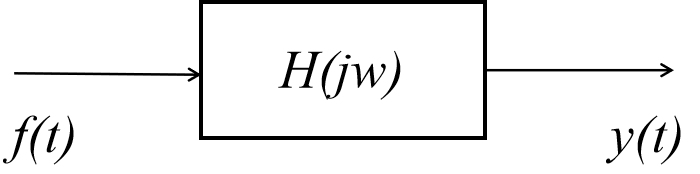
\includegraphics[width=0.45\linewidth]{assets/hw6img1.png}
			}
			\subfigure[]{
				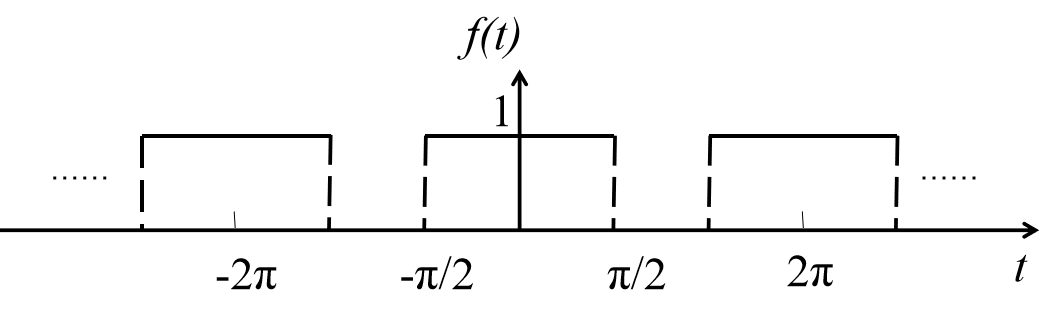
\includegraphics[width=0.45\linewidth]{assets/hw6img2.png}
			}
			
			\subfigure[]{
				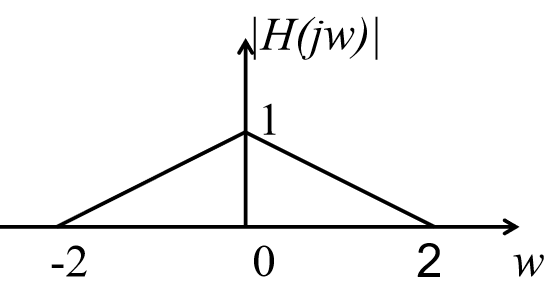
\includegraphics[width=0.45\linewidth]{assets/hw6img3.png}
			}
			\subfigure[]{
				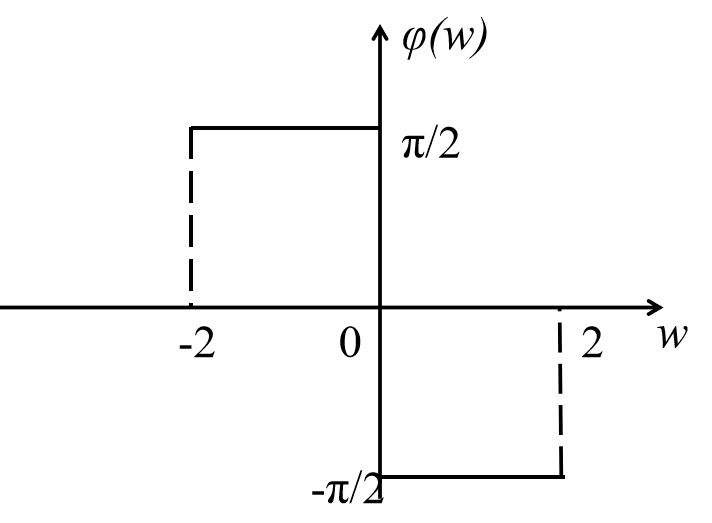
\includegraphics[width=0.45\linewidth]{assets/hw6img4.png}
			}
			\caption{}
			\label{fig:fig_micPerMon}
		\end{figure}
		\quad
	\end{problem}
	
	\newpage

	\begin{problem}
		已知线性时不变系统的输入$f(t)$如图2所示,系统的冲激响应$h(t) = e^{-2t}U(t)$,试求该系统的零状态响应$y_f(t)$。
		\begin{figure}[H]
			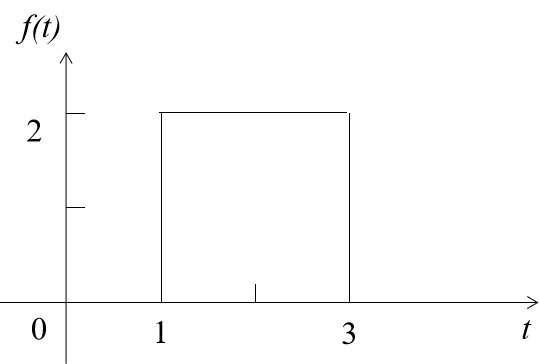
\includegraphics[width=0.7\linewidth]{assets/hw6_2.png}
			\centering
			\caption{}
		\end{figure}
		\quad
	\end{problem}

	\begin{problem}
		描述某线性时不变系统的方程为
		\newline
		$y^{''}(t) + 7y^{'}(t) + 12y(t) = f^{'}(t) + 2f(t)$,试:
		\begin{exercise}
			\task 求该系统的冲激响应$h(t)$;
			\task 若输入$f(t) = 6e^{-t}U(t)$,求系统的零状态响应$y_f(t)$。
		\end{exercise}	
		\quad
	\end{problem}
	\newpage
	
	\begin{problem}
		图3(a)为通信设备中常用的一抑制载波振幅调制的解调系统,其中低通滤波器的频响函数的幅频特性如图3(b)所示,相频特性$\varphi(w) = 0$。$s(t) = \cos(1000t)$,$-\infty < t < \infty$。若输入信号$f(t) = \frac{\sin t}{\pi t}\cos(1000t)$,$-\infty < t < \infty$,试求该系统的输出信号$y(t)$。
		\begin{figure}[htbp]
			\centering
			\subfigure[]{
				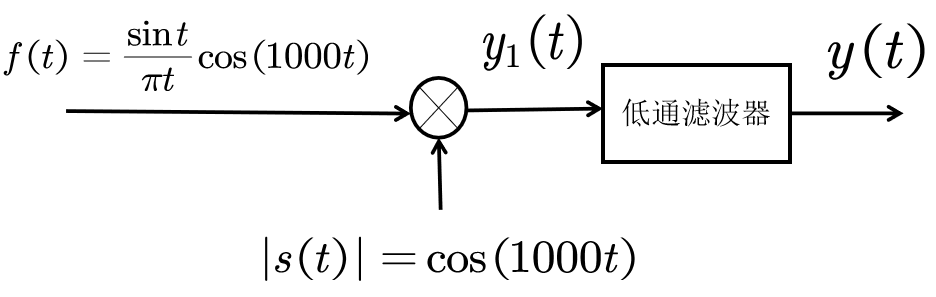
\includegraphics[width=0.9\linewidth]{assets/hw6_4_1.png}
			}
		
			\subfigure[]{
				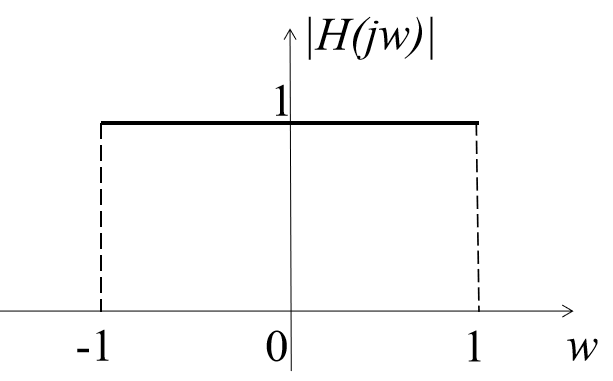
\includegraphics[width=0.7\linewidth]{assets/hw6_4_2.png}
			}
		\caption{}
		\end{figure}
	
		\quad
	\end{problem}
	
	
    \newpage
	\begin{problem}
		已知一个系统由图4所示4个子系统互联而成。其中:
		\newline
		$h_1(t)  = \frac{\mathrm{d}}{\mathrm{dt}}\big[\frac{\sin w_ct}{2\pi t}\big]$,$H_2(jw) = e^{-j2\pi w/w_c}$,$h_3(t) = \frac{\sin3w_ct}{\pi t}$,$h_4(t) = U(t)$。
		\newline
		若$f(t) = \sin2w_ct + \cos(w_ct/2)$,求系统的输出$y(t)$。
		\begin{figure}[H]
			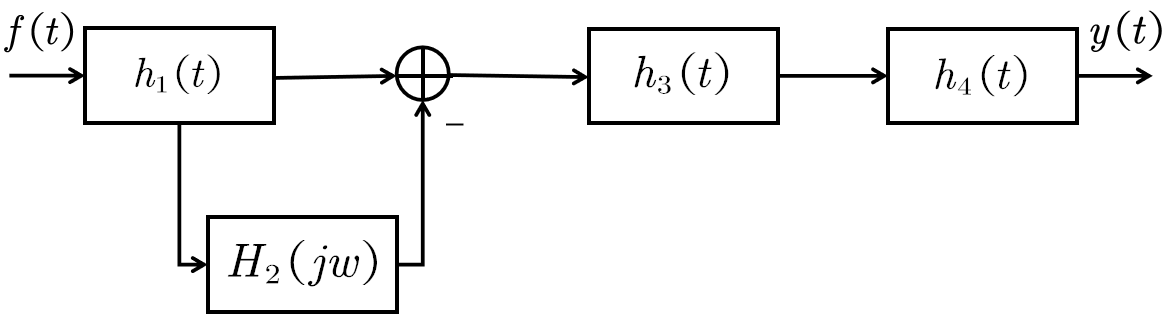
\includegraphics[width=0.95\linewidth]{assets/hw6_5.png}
			\centering
			\caption{}
		\end{figure}
		\quad
	\end{problem}
	
	\begin{problem}
		已知一个系统的框图如图5(a)所示:
		其中$\delta_T(t)$为周期冲激串函数信号,周期$T = 1$。若周期信号$f(t)$的波形如图5(b)所示,画出$y_f(t)$的频谱。
		\begin{figure}[htbp]
			\centering
			\subfigure[]{
				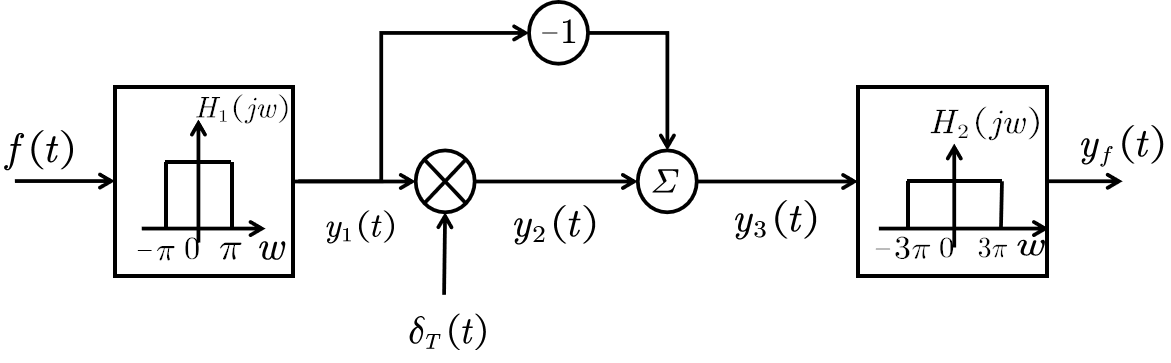
\includegraphics[width=0.95\linewidth]{assets/hw6_6_1.png}
			}
		
			\subfigure[]{
				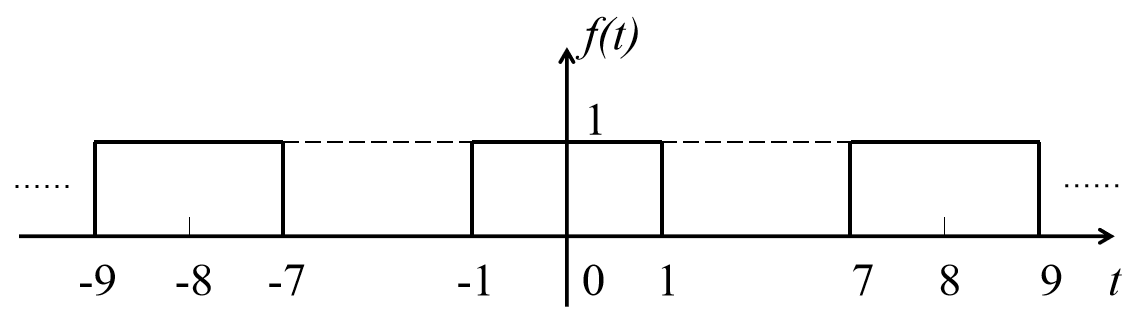
\includegraphics[width=0.7\linewidth]{assets/hw6_6_2.png}
			}
			\caption{}
		\end{figure}
		\quad
	\end{problem}
	
	\begin{problem}
		求图6所示电路的系统函数$H(jw) = \frac{U_2(jw)}{U_1(jw)}$。
		\begin{figure}[H]
			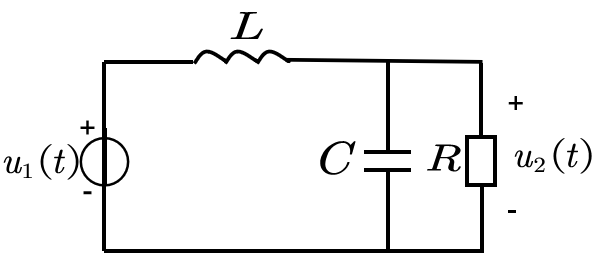
\includegraphics[width=0.6\linewidth]{assets/hw6_7.png}
			\centering
			\caption{}
		\end{figure}
		\quad
	\end{problem}
	
	\begin{problem}
		已知理想低通滤波器的传输函数$H(jw) = 5e^{-jwt_d}$,$|w| < 1$,激励$f(t) = 10e^{-t}U(t)$,如图7所示,求:
		\begin{exercise}
			\task $f(t)$的能量$W$;
			\task 响应$y(t)$的能量频谱函数$G(w)$。
		\end{exercise}
	\begin{figure}[H]
		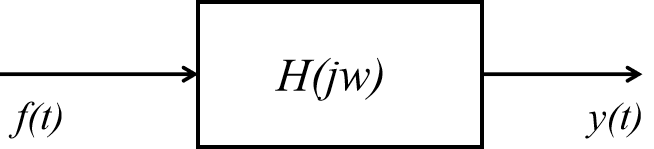
\includegraphics[width=0.6\linewidth]{assets/hw6_8.png}
		\centering
		\caption{}
	\end{figure}
		\quad
	\end{problem}

    \newpage
	\begin{problem}
		某一线性系统如图8(a)所示,输入信号$f(t)$的频谱$F(jw)$如图8(b)所示,它通过网络$H_1(w)$后便用冲激串$\delta_T(t)$进行抽样,$|H_1(jw)|$的特性如图8(c)所示。
		\begin{exercise}
			\task 为保证不出现混叠效应,求最低抽样频率$f_s$;
			\task 求抽样输出信号$y(t)$的频谱函数;
			\task 若抽样输出的脉冲调幅信号通过理想信道,为了使接收端能实现无失真地恢复原信号$f(t)$,问接入的网络$H_2(jw)$应具有什么样的特性。
		\end{exercise}
	\begin{figure}[H]
		\centering
		\subfigure[]{
			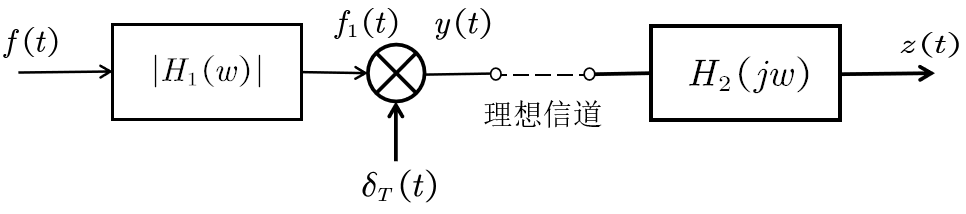
\includegraphics[width=0.95\linewidth]{assets/hw6_9_1.png}
		}
		
		\subfigure[]{
			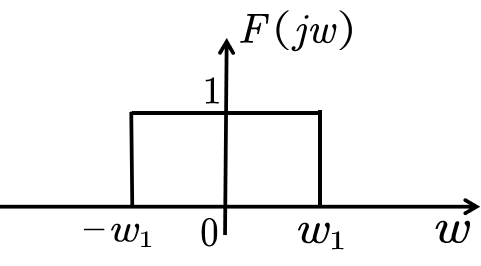
\includegraphics[width=0.45\linewidth]{assets/hw6_9_2.png}
		}
		\subfigure[]{
			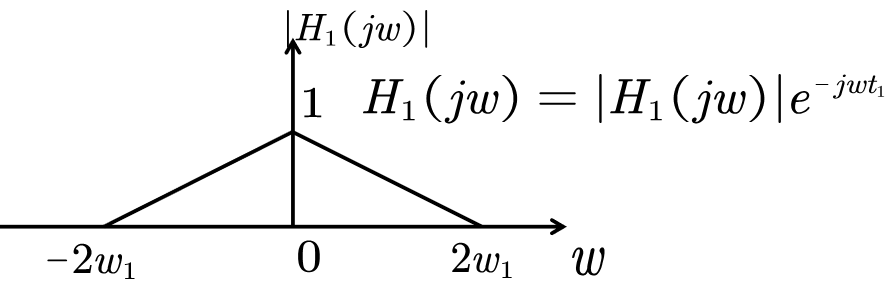
\includegraphics[width=0.45\linewidth]{assets/hw6_9_3.png}
		}
		\caption{}
	\end{figure}
		\quad
	\end{problem}

    \begin{problem}
    	一种多路复用系统如图9(a)所示,解复用系统如图9(b)所示。假定$f_1(t)$和$f_2(t)$都是带限信号,其最高频率为$w_M$,因此当$|w| > w_M$时,$F_1(jw) = F_2(jw) = 0$。假定载波频率$w_c$大于$w_M$,证明$y_1(t) = f_1(t)$,$y_2(t) = f_2(t)$。
    		\begin{figure}[H]
    		\centering
    		\subfigure[]{
    			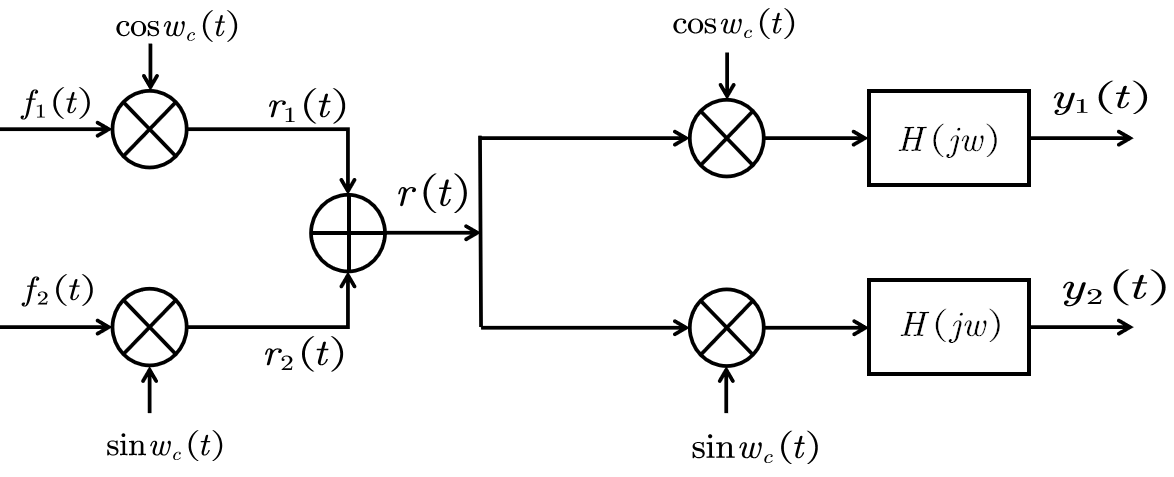
\includegraphics[width=0.95\linewidth]{assets/hw6_10_1.png}
    		}
    		
    		\subfigure[]{
    			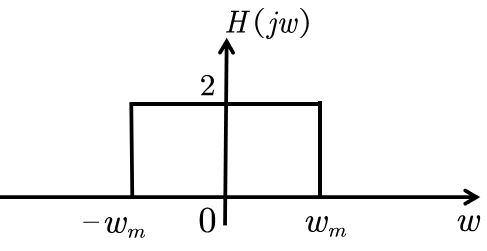
\includegraphics[width=0.7\linewidth]{assets/hw6_10_2.png}
    		}
    		\caption{}
    	\end{figure}
    \quad
    \end{problem}	
  
    \begin{problem}
    	$f(t) = \mathrm{Sa}(1000\pi t)\mathrm{Sa}(2000\pi t)$,$s(t) = \sum_{-\infty}^{\infty}\delta(t - nT)$,
    	\newline
    	$f_s(t) = f(t)s(t)$。
    	\begin{exercise}
    		\task 若要从$f_s(t)$无失真的恢复$f(t)$,求最大抽样周期$T_N$;
    		\task 当抽样周期$T = T_N$时画出$f_s(t)$的频谱图。
    	\end{exercise}
    
    	\quad
    \end{problem}

	\begin{problem}
		已知频域系统函数$H(jw) = \frac{jw}{-w^2 + j5w + 6}$,系统的初始状态$y(0) = 2$,$y^{'}(0) = 1$,激励$f(t) = e^{-t}U(t)$。求全响应$y(t)$。
	\end{problem}
	
\end{document}